\documentclass[10pt,a4paper]{article}
\usepackage[T1]{fontenc}
\usepackage[utf8]{inputenc}
\usepackage{lmodern}
\usepackage[margin=18mm,headheight=14pt]{geometry}
\usepackage{xcolor,graphicx,booktabs,tabularx,array,amsmath,amssymb}
\usepackage{tikz}
\usetikzlibrary{arrows.meta,positioning,calc}
\usepackage{hyperref,fancyhdr,enumitem}
\definecolor{ink}{HTML}{183247}
\definecolor{teal}{HTML}{117F80}
\definecolor{sky}{HTML}{E9F3F3}
\definecolor{amber}{HTML}{BB742E}
\definecolor{sand}{HTML}{FBF1E5}
\definecolor{muted}{HTML}{576977}
\definecolor{line}{HTML}{CEDCE0}
\definecolor{pale}{HTML}{F4F8FA}
\hypersetup{colorlinks=true,linkcolor=teal,urlcolor=teal,citecolor=teal,pdfauthor={Dharan Tej Reddy},pdftitle={Vision Mamba Diabetic Retinopathy: Implementation Dossier}}
\pagestyle{fancy}
\fancyhf{}
\fancyhead[L]{\small\color{muted}VISION MAMBA / RETINAL GRADING}
\fancyhead[R]{\small\color{muted}IMPLEMENTATION DOSSIER}
\fancyfoot[L]{\small\color{muted}4 November 2026}
\fancyfoot[R]{\small\color{muted}\thepage}
\renewcommand{\headrulewidth}{0.4pt}
\setlength{\parskip}{6pt}
\setlength{\parindent}{0pt}
\setlist[itemize]{leftmargin=15pt,itemsep=2pt,topsep=3pt}
\setlist[enumerate]{leftmargin=18pt,itemsep=2pt,topsep=3pt}
\newcommand{\tagline}[1]{\colorbox{sky}{\parbox{\dimexpr\linewidth-2\fboxsep}{\small #1}}}
\newcommand{\smallhead}[1]{\vspace{5pt}{\color{teal}\bfseries #1}\par}
\newcommand{\code}[1]{\texttt{\small #1}}
\newcolumntype{Y}{>{\raggedright\arraybackslash}X}
\begin{document}
\vspace*{12mm}
{\Large\color{teal}\bfseries RESEARCH IMPLEMENTATION / EVIDENCE RECORD}\par
\vspace{7mm}
{\Huge\color{ink}\bfseries Diabetic retinopathy grading\\[2mm] with Vision Mamba}\par
\vspace{5mm}
{\Large\color{muted}Architecture, data controls, verification and delivery status}\par
\vspace{10mm}
{\large Dharan Tej Reddy \hfill 4 November 2026}\par
\vspace{7mm}
\colorbox{sand}{\parbox{\dimexpr\linewidth-2\fboxsep}{\small
\textbf{Scope of this document.} This implementation dossier records the
code and preparation work. It is \textbf{not} the assignment's final experimental
report. A full training run, held-out classification metrics, prediction figures
and a result-bearing LaTeX report do not yet exist. Two recorded optimizer
steps are qualification checks only.}}\par
\vspace{7mm}
\smallhead{Project links}
\href{https://github.com/dharan1007/internship-task-1}{GitHub source repository}
\quad$\cdot$\quad
\href{https://arxiv.org/abs/2401.09417}{Vision Mamba paper}
\quad$\cdot$\quad
\href{https://www.kaggle.com/competitions/diabetic-retinopathy-detection/data}{Original EyePACS release}
\par
\vspace{7mm}

\begin{tikzpicture}[x=\linewidth,y=1cm]
 \fill[ink] (0,0) rectangle (1,0.13);
 \fill[teal] (0,0) rectangle (.72,0.13);
 \fill[amber] (.72,0) rectangle (1,0.13);
\end{tikzpicture}
\vfill
{\small\color{muted}Source code and documentation are public. Retinal images,
labels, credentials, private access links and diagnostic artifacts remain in
private storage.}
\newpage

\section*{\color{ink}1 \quad Assignment and delivery state}
The internship brief asks for a Vision Mamba classifier implemented from
scratch in PyTorch, a custom EyePACS \code{Dataset} used with
\code{DataLoader}, five-grade training, held-out EyePACS and Messidor
evaluation, metrics and example predictions, and a compiled LaTeX results
report. It evaluates code quality, architecture understanding, analysis,
documentation and reproducibility. The last two output groups still depend
on a completed experiment.

\small
\begin{tabularx}{\linewidth}{@{}p{.22\linewidth}Y p{.20\linewidth}@{}}
\toprule
Expected deliverable & Existing implementation & Evidence state\\
\midrule
PyTorch Vim & Own model blocks, reference and parallel scan, five-logit head &
Source exists; earlier revision passed two real-image optimizer steps\\
Dataset/preprocessing & Own retinal \code{Dataset}; full-field transform;
manifest, split and audit; PyTorch \code{DataLoader} &
35,126 original EyePACS images audited privately\\
Train/evaluate scripts & CLI, qualification, checkpointed training, sealed
evaluation, metrics and report generator &
Code tested; full epoch and sealed evaluation unrun\\
Metrics and predictions & Result generators reject incomplete runs &
No measured test results\\
Compiled results report & LaTeX generator and compiler smoke check &
No final experiment PDF\\
\bottomrule
\end{tabularx}
\normalsize

\tagline{For a code-focused review, the first three deliverables are available
as source. That is a reduced-scope submission against the PDF, because the
PDF also asks for real training and results.}


\section*{\color{ink}2 \quad Architecture and paper mapping}
The Vision Mamba paper represents images as sequences of position-marked
patches and uses selective state-space processing in both directions to build
global context \cite{vim}. This implementation uses a middle class token and
independent forward/reverse convolution and SSM parameters. It does not import
a ready-made Vim model or pretrained weights. The
\href{https://github.com/hustvl/Vim}{authors' implementation} informed the
architecture review, not the model dependency.

\begin{center}
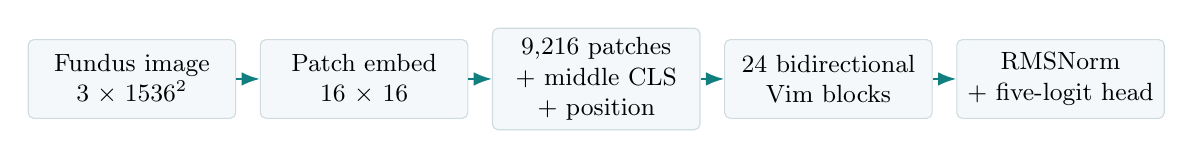
\begin{tikzpicture}[node distance=3mm, >=Latex,
 box/.style={draw=line,rounded corners=2pt,fill=pale,align=center,
            minimum height=10mm,text width=24mm,font=\small},
 arrow/.style={-Latex,thick,draw=teal}]
\node[box] (im) {Fundus image\\$3\times1536^2$};
\node[box,right=of im] (patch) {Patch embed\\$16\times16$};
\node[box,right=of patch] (tok) {9,216 patches\\+ middle CLS\\+ position};
\node[box,right=of tok] (blocks) {24 bidirectional\\Vim blocks};
\node[box,right=of blocks] (head) {RMSNorm\\+ five-logit head};
\draw[arrow] (im)--(patch); \draw[arrow] (patch)--(tok);
\draw[arrow] (tok)--(blocks); \draw[arrow] (blocks)--(head);
\end{tikzpicture}

{\small\color{muted}Figure 1. Implemented inference path. These are configured
dimensions, not a measured clinical operating point.}
\end{center}

For image side $H=1536$, patch side $P=16$, width $D=768$ and five grades,
the token count and shapes are
\[
N=(H/P)^2=96^2=9{,}216,\qquad L=N+1=9{,}217,
\]
\[
\mathrm{patch\ tokens}\in\mathbb{R}^{B\times N\times768},\qquad
\mathrm{class\ logits}\in\mathbb{R}^{B\times5}.
\]
The configured block uses expansion factor two, directional width $E=1{,}536$,
state dimension $S=16$, causal convolution width four, and depth 24. The
instantiated classifier has 103,760,645 trainable parameters. The
1536-pixel input and 300-epoch schedule are project choices, not settings
mandated by the paper or assignment brief.

\newpage
\section*{\color{ink}3 \quad Bidirectional selective state-space block}
Every block RMS-normalizes its input, projects features and a shared gate,
and processes the features forward and in reverse token order. Each
direction has its own causal depthwise convolution, input-dependent
state projections, step-size projection, negative diagonal state matrix
and skip coefficient. The outputs are returned to the original order,
summed, gated, projected and added to an FP32 residual.

\begin{center}
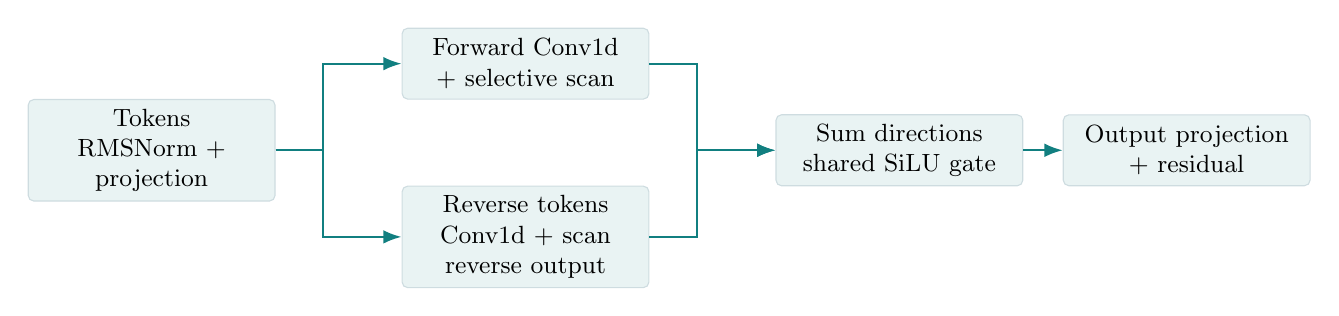
\begin{tikzpicture}[>=Latex, node distance=5mm,
 b/.style={draw=line,fill=sky,rounded corners=2pt,text width=29mm,
 align=center,minimum height=9mm,font=\small},
 a/.style={-Latex,thick,draw=teal}]
\node[b] (input) {Tokens\\RMSNorm + projection};
\node[b,right=16mm of input,yshift=11mm] (fwd) {Forward Conv1d\\+ selective scan};
\node[b,right=16mm of input,yshift=-11mm] (rev) {Reverse tokens\\Conv1d + scan\\reverse output};
\node[b,right=16mm of fwd,yshift=-11mm] (mix) {Sum directions\\shared SiLU gate};
\node[b,right=of mix] (out) {Output projection\\+ residual};
\draw[a] (input.east) -- ++(6mm,0) |- (fwd.west);
\draw[a] (input.east) -- ++(6mm,0) |- (rev.west);
\draw[a] (fwd.east) -- ++(6mm,0) |- (mix.west);
\draw[a] (rev.east) -- ++(6mm,0) |- (mix.west);
\draw[a] (mix)--(out);
\end{tikzpicture}

{\small\color{muted}Figure 2. The forward and reverse SSM/convolution
parameters are independent; the gate is shared.}
\end{center}

In the reference scan, $\Delta_t$ and $B_t,C_t$ depend on current input,
$A=-\exp(A_{\log})$, and the state update uses FP32:
\[
\bar A_t=\exp(\Delta_t A),\qquad
h_t=\bar A_t\odot h_{t-1}+\Delta_t B_t\odot x_t,\qquad
y_t=\langle C_t,h_t\rangle+D_{\rm skip}\odot x_t.
\]
The input drive follows the released Mamba/Vim selective-scan convention
$\Delta_t B_t$ \cite{mamba}. The primary parallel backend composes affine
transitions in bounded chunks and implements its own backward recurrence.
It does not reproduce the paper's fused SRAM kernel, so the paper's
published speedups are not claims about this implementation.

\small
\begin{tabularx}{\linewidth}{@{}p{.19\linewidth}Y p{.27\linewidth}@{}}
\toprule
Path & Purpose & Present evidence\\
\midrule
Reference & Transparent recurrence and gradient comparison &
Mathematical source; local parity tests\\
Parallel & Primary from-scratch PyTorch training path &
Earlier BF16 source passed real-image parity and two model steps\\
Pinned CUDA & Optional low-level scan efficiency path, never a ready-made Vim
model & Scan-only benchmark passed; current whole model unqualified\\
\bottomrule
\end{tabularx}
\normalsize

\smallhead{Implementation map}
\code{src/drvim/model/vim.py} defines the classifier, blocks and directional
mixers. \code{src/drvim/model/scan.py} defines the reference, in-house parallel
and optional pinned kernel paths. \code{src/drvim/qualify\_scan.py} compares
numerics and runs real-image optimizer preflight before training can accept
a qualification artifact.

\newpage
\section*{\color{ink}4 \quad Data architecture and leakage controls}
The original EyePACS training release has 35,126 labeled JPEGs. The
private preparation job read all five official archive parts, checked
archive CRCs, decoded and SHA-256 hashed every image, reconciled it to a
label, and assigned a grade-stratified split that keeps filename-paired
left and right eyes together.

\begin{center}
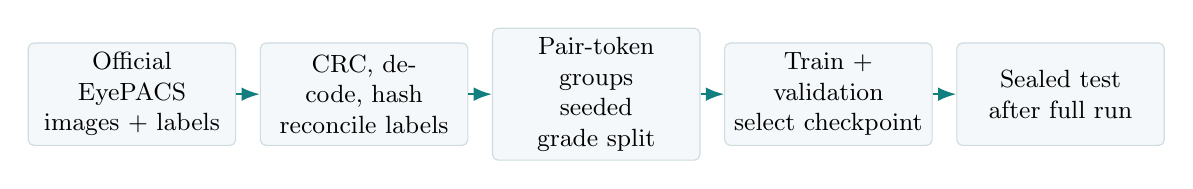
\begin{tikzpicture}[>=Latex,node distance=3mm,
 b/.style={draw=line,rounded corners=2pt,fill=pale,text width=24mm,
 align=center,minimum height=13mm,font=\small},
 a/.style={-Latex,thick,draw=teal}]
\node[b] (src) {Official EyePACS\\images + labels};
\node[b,right=of src] (audit) {CRC, decode, hash\\reconcile labels};
\node[b,right=of audit] (split) {Pair-token groups\\seeded grade split};
\node[b,right=of split] (dev) {Train + validation\\select checkpoint};
\node[b,right=of dev] (test) {Sealed test\\after full run};
\draw[a] (src)--(audit); \draw[a] (audit)--(split);
\draw[a] (split)--(dev); \draw[a] (dev)--(test);
\end{tikzpicture}

{\small\color{muted}Figure 3. Preparation and test boundary. Filename
pairing tokens do not independently prove unique patient identity.}
\end{center}

\begin{center}
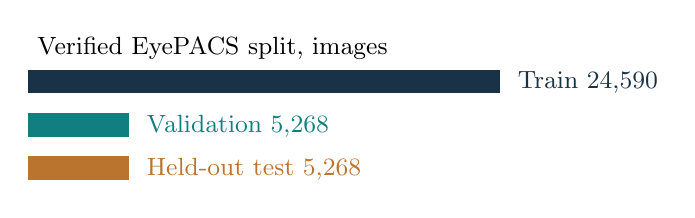
\begin{tikzpicture}[x=0.00025cm,y=0.55cm]
\fill[ink] (0,2.3) rectangle (24590,2.85);
\fill[teal] (0,1.3) rectangle (5268,1.85);
\fill[amber] (0,.3) rectangle (5268,.85);
\node[anchor=west,font=\small] at (0,3.35) {Verified EyePACS split, images};
\node[anchor=west,font=\small\color{ink}] at (25000,2.55) {Train 24,590};
\node[anchor=west,font=\small\color{teal}] at (5700,1.55) {Validation 5,268};
\node[anchor=west,font=\small\color{amber}] at (5700,.55) {Held-out test 5,268};
\end{tikzpicture}
\end{center}

The active custom \code{RetinaDataset} loads records for its declared
source and split. Its transform applies EXIF orientation, converts to RGB,
rescales without cropping the retinal field, pads to a square, and allows
horizontal flipping only for training. PyTorch's \code{DataLoader} supplies
workers and batching; no ready-made retinal dataset loader is used.

A separate high-assurance candidate adds pinned manifest identity, per-read
byte hashing, size and format limits, ICC-to-sRGB conversion, deterministic
augmentation, and metadata evidence gates. It is \textbf{not connected to
the primary training run}. The public EyePACS release lacks verified
patient linkage, site, camera, acquisition date, adjudication and rights
metadata; the candidate mode therefore fails closed instead of inventing
those fields.

\small
\begin{tabularx}{\linewidth}{@{}p{.24\linewidth}Y Y@{}}
\toprule
Concern & Active assignment loader & Optional high-assurance candidate\\
\midrule
Source identity & Manifest checked before run & Manifest pinned and image
bytes rehashed at sample read\\
Color & RGB conversion & Embedded ICC to sRGB; untagged assumption recorded\\
Geometry & Full-field letterbox & Same geometry plus occupancy metadata\\
Augmentation & Train-only random flip & Seed/epoch/image-ID deterministic flip\\
Clinical metadata & Unavailable & Explicit patient/site/device/grade/rights
attestations required\\
\bottomrule
\end{tabularx}
\normalsize

\smallhead{Source map for data handling}
\small
\begin{tabularx}{\linewidth}{@{}p{.34\linewidth}Y@{}}
\toprule
File & Responsibility\\
\midrule
\code{data/prepare.py}, \code{data/manifest.py} &
Official cohort adapters, labels, hashes and strict manifest schema\\
\code{data/split.py}, \code{data/audit.py} &
Grouped assignment and leakage/source checks\\
\code{data/dataset.py}, \code{data/preprocess.py} &
Active custom Dataset and full-field image transform\\
\code{data/high\_assurance\_dataset.py} &
Separate candidate for stronger provenance and image controls\\
\bottomrule
\end{tabularx}
\normalsize

\smallhead{Official original Messidor preparation}
All 12 archives and 12 canonical annotation workbooks passed private
integrity checks. The preparer decoded and SHA-256 hashed 1,200 TIFFs,
applied four published grade corrections, and excluded 13 published
Base33 duplicates. Its schema-valid manifest has 1,187 eligible external
images: R0 547, R1 149, R2 240 and R3 251. Included image SHA-256 sets
have zero exact overlap with the verified EyePACS manifest; near duplicates
are not excluded by this check. No external model predictions exist.

\newpage
\section*{\color{ink}5 \quad Training and external evaluation}
The classifier is randomly initialized. The training code defines
cross-entropy, AdamW with parameter-specific decay exclusions, warmup and
cosine learning rate, mixed precision, gradient clipping, accumulation,
activation checkpointing and distributed data parallel execution. Each
completed epoch saves model, optimizer, scheduler, scaler, RNG, config and
manifest identity. Highest EyePACS validation QWK selects the checkpoint.
The held-out EyePACS and Messidor tests never select hyperparameters.
\[
\mathcal{L}_{\rm CE}
=-\frac{1}{M}\sum_{i=1}^{M}\log p_{\theta}(y_i\mid x_i),
\qquad y_i\in\{0,1,2,3,4\}.
\]
Distributed padding examples have zero contribution so each real training
image contributes once to the global loss. An epoch-boundary pause saves
a checkpoint without writing the full-run completion marker.

\smallhead{Declared configuration (not a completed run)}
\small
\begin{tabularx}{\linewidth}{@{}p{.23\linewidth}Y p{.23\linewidth}Y@{}}
\toprule
Setting & Value & Setting & Value\\
\midrule
Epochs / seed & 300 / 2026 & Batch / accum. & 2 / 4 per GPU\\
AdamW learning rate & $10^{-4}$ & Decay / warmup & 0.05 / 5 epochs\\
Precision & FP16 AMP & Clipping / drop path & 1.0 / 0.1\\
Workers per rank & 8 & Selection criterion & Validation QWK\\
\bottomrule
\end{tabularx}
\normalsize

Original Messidor is the external dataset named by the brief. Its R0--R3
grades differ from EyePACS ICDR 0--4; five-class QWK against original
Messidor would be invalid. The declared cross-source binary proxy is
Messidor R2/R3 versus model ICDR 2/3/4. Optional Messidor-2 uses separately
published adjudicated grades 0--4 \cite{messidor,adcis2}. Neither external
cohort enters training or checkpoint selection. ADCIS states that 1,058
Messidor-2 PNGs come from original Messidor and 690 JPGs form an extension;
the two named cohorts are therefore not independent replications.

The evaluation command requires a completed-run marker, pins the source
manifest and selected checkpoint, verifies images, then records per-image
probabilities and predictions. It calculates accuracy, precision, recall,
F1, QWK where valid, confusion matrices and loss curves. The report generator
recomputes metrics from saved rows before placing plots and image pairs in
LaTeX. \textbf{These generators exist; no classification results have been
generated yet.}

\smallhead{Declared metric definitions}
For a five-grade cohort, the confusion matrix contains integer counts
$C_{ij}=\#\{n:y_n=i,\hat y_n=j\}$. Accuracy is the fraction of correct
predictions; class precision, recall and F1 are computed with explicit
support. Macro values average the five class values equally. Quadratic
weighted kappa is
\[
\kappa_{\rm QW}=1-
\frac{\sum_{i,j}w_{ij}O_{ij}}{\sum_{i,j}w_{ij}E_{ij}},
\qquad
w_{ij}=\frac{(i-j)^2}{(K-1)^2},\quad K=5,
\]
where $O$ is observed grade-pair frequency and $E$ is the expected frequency
from the observed marginals. Undefined QWK is rejected rather than replaced
with a fabricated zero. Original Messidor receives its declared binary
endpoint only; five-grade QWK is reserved for commensurate ICDR labels.

\begin{center}
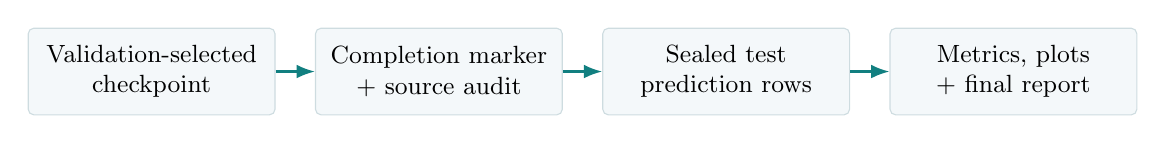
\begin{tikzpicture}[>=Latex,node distance=5mm,
 b/.style={draw=line,rounded corners=2pt,fill=pale,text width=29mm,
 align=center,minimum height=11mm,font=\small},
 a/.style={-Latex,thick,draw=teal}]
\node[b] (ckpt) {Validation-selected\\checkpoint};
\node[b,right=of ckpt] (seal) {Completion marker\\+ source audit};
\node[b,right=of seal] (pred) {Sealed test\\prediction rows};
\node[b,right=of pred] (metric) {Metrics, plots\\+ final report};
\draw[a] (ckpt)--(seal); \draw[a] (seal)--(pred); \draw[a] (pred)--(metric);
\end{tikzpicture}

{\small\color{muted}Figure 5. Implemented result gate. The rightmost
artifacts cannot exist honestly until the preceding experimental stages
complete.}
\end{center}


\newpage
\section*{\color{ink}6 \quad What has actually run}
\small
\begin{tabularx}{\linewidth}{@{}p{.27\linewidth}Y p{.18\linewidth}@{}}
\toprule
Check & Observed result & Interpretation\\
\midrule
Original EyePACS preparation & 35,126 labeled images decoded and hashed;
all five grades in each split; no filename-pair group crosses splits &
Complete data audit, not model training\\
Earlier BF16/parallel qualification & One Tesla T4, 1536-pixel input,
103,760,645 parameters; two eight-image optimizer steps of 195.71 and
197.24 seconds; peak allocation 4.64 and 5.47 GB &
Two-step diagnostic only\\
Scan-only comparison & At 9,217 tokens on T4, in-house FP32 scan 0.334 s
versus pinned CUDA scan 0.0256 s; forward maximum absolute difference
$1.31\times10^{-6}$ &
About 13 times faster for this scan benchmark only\\
Repository checks & Ruff passed and 12 local tests passed &
Source checks, not accuracy\\
\bottomrule
\end{tabularx}
\normalsize

\begin{center}
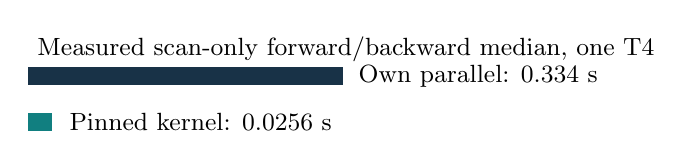
\begin{tikzpicture}[x=12cm,y=.45cm]
\node[anchor=west,font=\small] at (0,3.1) {Measured scan-only forward/backward median, one T4};
\fill[ink] (0,2.1) rectangle (.334,2.6);
\fill[teal] (0,.8) rectangle (.0256,1.3);
\node[anchor=west,font=\small] at (.34,2.35) {Own parallel: 0.334 s};
\node[anchor=west,font=\small] at (.034,1.05) {Pinned kernel: 0.0256 s};
\end{tikzpicture}

{\small\color{muted}Figure 4. This compares only a selective-scan direction,
not a complete model step, epoch or classifier.}
\end{center}

The kernel timing does not establish full-model throughput. The two-step
qualification is pinned to an earlier BF16/parallel source revision. The
current FP16/optional CUDA code requires its own exact-source qualification.
At the earlier T4 rate, the configured 300-epoch experiment cannot fit the
available free Kaggle time budget. The brief does not require 300 epochs.
No paid environment has been used.

\section*{\color{ink}7 \quad Stack and reproducibility}
\small
\begin{tabularx}{\linewidth}{@{}p{.27\linewidth}Y@{}}
\toprule
Technology & Role and boundary\\
\midrule
Python 3.10+ & Package, CLI, manifests and acquisition verification\\
PyTorch & Tensors, autodiff, \code{Dataset}/\code{DataLoader}, AMP, DDP and
layers; model and training loop are authored in this repository\\
NumPy / pandas & Array conversion, annotation tables and manifests\\
Pillow & JPEG/TIFF decode, EXIF correction, resize and optional color control\\
scikit-learn & Metrics and confusion counts, not a ready-made retinal model\\
Matplotlib & Plots only after actual evaluation\\
PyYAML & Recorded experiment configuration\\
xlrd / openpyxl & Official Messidor workbook parsing\\
Tectonic / pdfLaTeX & Result report compilation\\
Kaggle & Private EyePACS input and GPU diagnostic jobs\\
Git / GitHub & Public source and docs; no images, credentials or weights\\
\bottomrule
\end{tabularx}
\normalsize

The public repository is
\href{https://github.com/dharan1007/internship-task-1}{github.com/dharan1007/internship-task-1}.
The audited EyePACS split manifest SHA-256 is
{\scriptsize\code{f933f1bcff8f99688fd8a44984acaa4ce0c929d899be9bddcabdfc54ea7c2117}}.
The hash identifies the exact split; raw licensed images remain private.
Source, manifest, config, checkpoint and report artifact identities are
recorded so a finished experiment can be traced back to its inputs.


\newpage
\section*{\color{ink}8 \quad Access and support timeline}
\small
\begin{tabularx}{\linewidth}{@{}p{.22\linewidth}Y@{}}
\toprule
Date & Recorded event\\
\midrule
3 November 2026 & Requested exact-scope EyePACS internship use and
image-in-report permission. Submitted ADCIS Messidor and Messidor-2
access forms and contacted ADCIS support when personal links did not arrive.\\
4 November 2026 & EyePACS contact directed use of its Kaggle release and
requested EyePACS, Inc. and Cuadros--Bresnick (2009) credit. This did not
expressly settle every proposed training, weight-sharing and image-report
scope.\\
4 November 2026 & Original EyePACS audit and grouped split completed in
private storage. Earlier model two-step qualification and separate CUDA
scan comparison completed on Kaggle.\\
4 November 2026 & ADCIS technical support replied with restricted
alternative access for original Messidor and Messidor-2 after the form
issue. Private links and credentials are omitted here.\\
4 November 2026 & All 12 original Messidor archives passed private size,
hash and ZIP checks. The 1,200 TIFFs and 12 canonical annotation workbooks
yielded a schema-valid manifest with 1,187 eligible images after 13
published duplicate exclusions.\\
4 November 2026 & Four official Messidor-2 image parts passed byte-size and
hash checks. The assembled ZIP passed CRC; all 1,748 extracted images passed
full decode and byte-hash uniqueness checks. Official pairing is unresolved.\\
4 November 2026 & Compared the block with Vim Algorithm 1 and corrected
directional combination to a sum before the shared gate and projection.
Earlier GPU qualification does not certify this revised source.\\
\bottomrule
\end{tabularx}
\normalsize

The official
\href{https://www.adcis.net/en/third-party/messidor/}{Messidor} and
\href{https://www.adcis.net/en/third-party/messidor2/}{Messidor-2}
pages permit free research and educational use while prohibiting copying
and redistribution. They request acknowledgment of the Messidor program
(``Kindly provided by the Messidor program partners'') and, for Messidor-2,
the LaTIM laboratory \cite{messidor,adcis2,abramoff}.
Restricted access details and images are not in
this dossier or the public repository.

\section*{\color{ink}9 \quad Kaggle evidence and source links}
\begin{enumerate}
\item \href{https://www.kaggle.com/code/dharantejreddy/drvim-prepare-original-eyepacs}
{Prepare Original EyePACS}: official-source preparation, 35,126 JPEGs
decoded and hashed, label reconciliation and fixed split. Produced the
manifest used for subsequent qualification.
\item \href{https://www.kaggle.com/code/dharantejreddy/drvim-full-model-qualification}
{Full Model Qualification}: checked FP32/BF16 scan parity and executed
two complete optimizer steps on real EyePACS images under the pinned
full-split identity. It is not an epoch or validation measurement.
\item \href{https://www.kaggle.com/code/dharantejreddy/drvim-pinned-cuda-scan-build}
{Pinned CUDA Scan Build}: built a pinned low-level selective-scan wheel in
the Kaggle environment, with no pretrained weights.
\item \href{https://www.kaggle.com/code/dharantejreddy/drvim-real-eyepacs-cuda-scan-comparison}
{Real EyePACS CUDA Scan Comparison}: compared the in-house scan and the
low-level kernel on real-image-derived inputs at intended token length.
Reports kernel-level timing and numerical differences, not classifier
accuracy or whole-model runtime.
\end{enumerate}
These notebooks may require owner access. None is a live full training job.

\newpage
\section*{\color{ink}10 \quad Remaining work and limits}
\begin{enumerate}
\item Run the exact-source and cross-cohort audit with the completed original
Messidor manifest before sealed inference. The verified images and manifest
alone are not external model results.
\item Requalify the current FP16 and optional CUDA full-model source,
measure a complete epoch and distributed throughput, and find a zero-cost
allocation that can finish a predeclared training schedule.
\item Train five-grade classification fully, selecting the checkpoint on
EyePACS validation only. Preserve checkpoint and run identity.
\item Run sealed held-out EyePACS and original Messidor evaluation; generate
measured metrics, plots and real example predictions. Add Messidor-2 only
after its official images and pairing metadata are reconciled.
\item Compile and inspect the final \emph{results} LaTeX report. Confirm
applicable EyePACS permission before sharing image-bearing PDFs or weights.
\end{enumerate}
This is research software, not a medical device or clinical diagnostic
claim. Public EyePACS filenames do not independently prove patient identity.
Acquisition, quality, grading-standard and population differences may
affect external generalization.

\begin{thebibliography}{10}\small
\bibitem{vim} L. Zhu et al., "Vision Mamba: Efficient Visual Representation
Learning with Bidirectional State Space Model," ICML 2024.
\url{https://arxiv.org/abs/2401.09417}.
\bibitem{mamba} A. Gu and T. Dao, "Mamba: Linear-Time Sequence Modeling
with Selective State Spaces," 2023.
\url{https://arxiv.org/abs/2312.00752}.
\bibitem{eyepacs} J. Cuadros and G. Bresnick, "EyePACS: An Adaptable
Telemedicine System for Diabetic Retinopathy Screening," \emph{Journal of
Diabetes Science and Technology}, 3(3):509--516, 2009. EyePACS, Inc. is
credited for the original
\url{https://www.kaggle.com/competitions/diabetic-retinopathy-detection/data}
retinal image release.
\bibitem{messidor} E. Decencière et al., "Feedback on a publicly
distributed database: the Messidor database," \emph{Image Analysis \&
Stereology}, 33(3):231--234, 2014. Kindly provided by the Messidor
program partners. \url{https://www.adcis.net/en/third-party/messidor/}.
\bibitem{adcis2} Messidor program partners, "Messidor-2" access and
acknowledgment. \url{https://www.adcis.net/en/third-party/messidor2/}.
\bibitem{abramoff} M. D. Abr\`amoff et al., "Automated analysis of retinal
images for detection of referable diabetic retinopathy," \emph{JAMA
Ophthalmology}, 131(3):351--357, 2013.
\url{https://doi.org/10.1001/jamaophthalmol.2013.1743}.
\bibitem{grades} Google Brain, "Messidor-2 DR Grades."
\url{https://www.kaggle.com/datasets/google-brain/messidor2-dr-grades}.
\end{thebibliography}
\end{document}
